\documentclass{llncs2e/llncs}
\usepackage{llncs2e/llncsdoc}

\usepackage{hyperref}
\usepackage{url}
\usepackage{graphics, graphicx}
\usepackage{caption}
\usepackage{csquotes}
\usepackage{balance}       % to better equalize the last page
\usepackage{graphics}      % for EPS, load graphicx instead 
\usepackage[T1]{fontenc}   % for umlauts and other diaeresis
\usepackage{txfonts}
\usepackage{mathptmx}
\usepackage{color}
\usepackage{booktabs}
\usepackage{textcomp}



\title{On the Impact of Adaptive Hints}

\author{Zhen Zhai\inst{1} \and Yoav Freund\inst{2}}
\institute{UC San Diego \email{zzhai@eng.ucsd.edu} \and UC San Diego \email{yfreund@eng.ucsd.edu}}

\begin{document}
\maketitle

%%%%%%%%%%%%%%%%%%%%%%%%%%%%%%%%%%%%%%%%%%%%%%%%%%%%%%%%%%%%%%%%%%%%%%%%%%%%%%%%
\begin{abstract}

We study the impact of an adaptive hint system that we designed to
help students as they are working on online assignments for a
probability and statistics course.

We report on a controlled experiment we performed to test whether
receiving hints improves student performance. We conclude with the
support from our experimental results. Our main main positive finding
is that students that receive a hint while solving a problem in an
assignment take significantly shorter time and fewer attempts to solve
later problems in the same assignment. This shows that hints have a
long term effect on students performance.

\end{abstract}


%%%%%%%%%%%%%%%%%%%%%%%%%%%%%%%%%%%%%%%%%%%%%%%%%%%%%%%%%%%%%%%%%%%%%%%%%%%%%%%%

\section{Introduction}

%\cite{ElkherjFreund14} described a system for delivering hints in the context of a web-based homework system. In the work presented here, we describe a controlled experiment that we have done in the context of an undergraduate course in probability and statistics. Our statistical analysis provides new evidence that adaptive hints are effective.


\subsection*{Background}
The goal of Intelligent tutoring systems (ITS)\cite{Anderson1995} is to imitate a human tutor.  ITS systems detect and classify student errors and provide instantaneous feedback intended to help students
understand and correct their error. The goal is to improve
student's understanding and improve their performance on {\em future} problems, rather than ``feeding'' them the answer to the current problem.  Previous research suggests that a computer tutor can nearly be as effective as a human tutor\cite{Vanlehn2011}. Hence, many intelligent tutors have been developed and introduced into classrooms. A few well developed ITS designed for algebra curriculum in middle school and high school mathematics has already been proven
to be effective\cite{Koedinger1997,John2014}.

Research has suggested that ``Formative'' feedback is essential to improving the learning process\cite{Azevedo1995}\cite{Bangert-Drowns1991}. Formative feedback is feedback that aims to improve students learning and is presented in the form of a response to student incorrect answers\cite{Shute2008}. According to Shute~\cite{Shute2008}, formative feedback needs to be specific, clear and timely. Furthermore, formative feedback should provide learners with both verification and elaboration \cite{Mason2001} \cite{Bangert-Drowns1991}. Verification is to provide feedback to learners as to whether the answer is correct or not. Elaboration is to provide a short elaboration on the topic or discuss the learner's incorrect answer. The timing of the feedback is important as well, Kulhavy and Anderson suggest that delayed feedback is better than instance feedback\cite{Kulhavy1972}. The adaptive hint system delay hints by only providing hints to students who have spent a certain amount of time on the problem without solving it. This allows the hints only go to students who are struggling with a problem. Finally, studies show that hint-on-demand allow students to learn more as compared to proactive hints\cite{Razzaq2010}. Therefore, the adaptive hint system is designed that a student will only see a hint if they click the 'Show Hint' button.

Homework is an essential part of students' learning process\cite{Cooper2006}. It gives students a chance to practice. Even more importantly, it allows them to identify their confusions and resolve them. There are many popular web-based homework systems for college students(e.g., WebAssign, WebWork, OWL, Andes). The goal is to help instructors to have a better management of a large enrollment class. These homework systems often provide feedback to students and provide analysis of student performance to instructors. Research has proven the web-based homework(WBH) systems to be helpful in learning\cite{MestHartRath2002}\cite{Vanlehn2005}. In these studies, the WBH systems, OWL and Andes, provide students with immediate feedback and hints following an incorrect attempt\cite{MestHartRath2002}\cite{Vanlehn2005}. The feedback and hints are the essential part of a WBH system, which is what our study focuses on.

\subsection*{Gaming the hint system}

A common concern regarding hint systems is the ability of students to game the system and extract the correct answer without understanding it\cite{Baker2004}\cite{Baker2005}. In previous studies, students have been shown to game the system by manipulating the tutoring system into giving out correct answers\cite{Baker2004Off-task}. As a result, students succeed in homework but fail on learning.

We avoid the gaming issue by combining three design principles.
First, the number of possible answers to each question is very large (typically more than 1000) making guessing the correct answer impractical.  Second, the information contained in the hint
identifies only the reason that the current answer is incorrect, it
does not identify the correct answer. Third, the hint contains a
simple question designed to highlight the mistake made by the student, so that by correctly answering the hint the student would realize the error in their thinking and be able to apply that knowledge to the original question.


\iffalse
our hints don't contain correct answers in any form. The adaptive hint
system generates short simple questions as hints instead of
 Therefore, we
replaced worked examples with short questions that are designed to
promote thinking and guide student's learning process. This resolve
the concern of students gaming the system because our system gives
students hints on how to learn instead of how to answer a specific
question. The only way for a student to obtain correct answers is by
learning how to solve the problem. Therefore, we not only prevent any
system gaming, but our hints also help students in long
term. Furthermore, our hint system targets mathematic problems, which
require students to type in mathematic expressions. Therefore, unlike
multiple choice problems, it would be nearly impossible to guess the
answer by looking at hints. There is infinity many ways one can type
in a mathematic expression and it is very hard for students to simply
guess it correctly with the help of hints. Therefore, we don't have
the concern of students gaming the system.
\fi

\subsection*{Contribution}

The main contribution of this paper is a demonstration, with high
statistical significance, that hints improve students
learning. Specifically, we show that students who receive a hint at a
point of time are likely to perform better on problems attempted
later. On the other hand, we detect no significant effect on
performance on the problem for which the hint was given (immediate
effect) nor on the performance of the student in the final exam.

\section*{Setup}

We extended and deployed the adaptive hint system described
in~\cite{ElkherjFreund14}.

The adaptive hint system is built on top of Open edX, an open source
MOOC platform. We used Open edX as our homework system and embedded
the adaptive hint system on top. The edX homework system prompts
students to answer problems by entering mathematical expressions and
provides instant feedback on the correctness of the answer. The
adaptive hint system provides additional feedback in the form of a
hint. Students receive one assignment per week. Each assignment
contains 5 to 10 problems and each problem has 1 to 10 parts. The
problems in an assignment all target similar material that is covered
in lecture. Students have an unlimited number of attempts for each
problem, they can spend as many attempts as they want until they get
to the correct answer.

The system was deployed in an undergraduate probability and statistic
class of around 300 students of which 245 participated in the
study. The hint system was used for 4 out of the eight assignments in
the course (other assignment were either too simple or did not lend
themselves to our methodology). There were a total of 26 problems and
each problem has between 1 to 10 questions each requiring student
response.

Significant work went into the careful design of 162 hints by the
course staff consisting of an instructor, four TAs, and four
tutors. The hints were designed based on historical data. Students
received a total of 3621 hints during these four weeks.

\section*{Design of the adaptive hint system}

Our adaptive hint system is based on a database of hints populated
manually before each assignment is released, based on historical
data~\footnote{Our system allows adding hints in real-time, however,
  doing so proved impractical.}. Each hint consists of the
following three parts:
\begin{enumerate}
\item {\bf Trigger:} a condition on the student's attempt that will
  cause the hint to be sent.
\item {\bf Message:} A message to the student identifying what is
  wrong in the attempt.
\item {\bf Question:} A simple question designed to help the student understand their mistake. Together with the correct answer to the question.   
\end{enumerate}


Following the work of Kulhavy and Anderson\cite{Kulhavy1972} we prefer not to give students the hint immediately and instead allow them to try to solve the problem on their own. to that end, the system delays sending the hint until the student spent on it 5 minutes or made at least 3 attempts.

Furthermore, students need to demand hints by clicking the "Show Hints" button. Hint-on-demand is suggested to be more effective than proactive hints\cite{Razzaq2010}. Once a hint is assigned to a student, the student can choose to click or not click the "Show Hint" button. One can ignore the assigned hint by not clicking the "Show Hint" button. If a student wants to see the assigned hint, he/she needs to click the "Show Hint" button to see the hint. In other words, we only show hints to students who ask for hints. Students who don't click the "Show Hints" button will not see the assigned hints. This makes sure we give on-demand hints to students who want help and are likely to spend time reading and understanding the hint.  In our analysis, we use this button-press to identify when the student read the hint.

A popular type of hint is a
worked-out-examples~\cite{Atkinson2000}. However, work by
Mclaren~\cite{McLaren2006} finds no significant effects of
worked-out-examples on learning in a web-based intelligent tutoring
environment. Therefore, the adaptive hint system gives students a
simple question to work on, instead of giving out
worked-example. Students can choose whether or not to answer the hint
question. If students choose to answer the hint question, the system
provides instant feedback to let the students know whether their
answers are correct or not. We make it clear to the students that
hints will not effect their grade. In particular, the student does not
have to click on ``Show Hint'' or to answer the question associated
with the hint.

\subsection*{Hints}

Our system supports two types of hints, generic and specific. Generic hints are triggered by an elementary problem with common error, while specific hints point to a particular type of error that occurs in a particular problem. Specific hints are usually based on finding an error in a mathematical expression using parsing, as will be explained below.

Some of the generic hints point out simple errors such as ``The size of a set cannot be negative'' or ``A probability cannot be large than 1''. Another generic hint is sent when a student gives an incorrect answer, and that answer is a number, rather than an expression. The system will ask students to write an expression instead of a number. Expression exposes more of the student's thinking process and allows specific hints to be sent.

Specific hints are sent based on the parsing of a mathematical
expression, as explained in the next section. The specific hint
directs the student to focus on the incorrect part of her answer.  In
addition, the hint usually includes a question. Answering this
question, while not compulsory, is designed to help the student
think about a similar problem in a simplified setting.

As an example of a specific hint, consider a problem about the
probability of a specific hand in a Texas Hold'em poker. Figure
\ref{fig:hint_prob} shows the problem, and Table \ref{tab:hints_sent}
shows some of the hints sent for this problem.

\begin{figure}[ht]
  \centering
	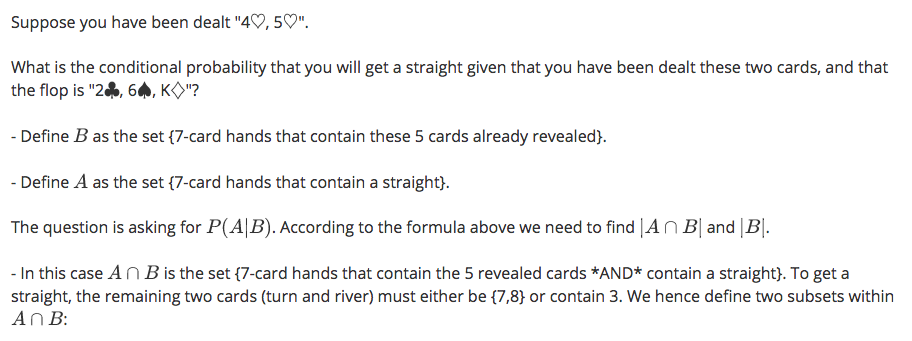
\includegraphics[width=0.95\textwidth]{image/problem_screenshot.png} \\
	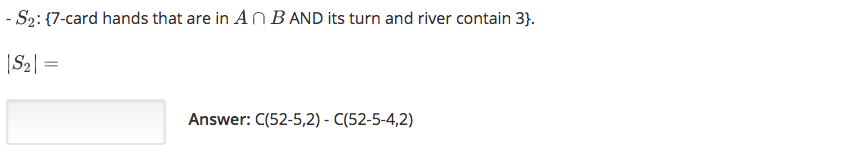
\includegraphics[width=0.95\textwidth]{image/part_screenshot.png}
   \caption{This is a problem(problem 5) assigned to students in
     week4. The problem is to find the probability of a specific hand
     in Texas Hold'em poker. This problem has four parts that students
     need to answer. The picture shows the second part.}
   \label{fig:hint_prob}
\end{figure}

\begin{table}[h]
\caption{The table listed some student attempts for one question of
  problem 5 in week 4 assignment. The problem is shown in Figure
  \ref{fig:hint_prob} along with the question of part 2 and
  solution. The first three hints are generic hints. The fourth
  attempt has no matching to any part of the solution, therefore the
  hint asks the student to first focus on the first part of the
  solution, which is $C(52-2,2)$. This hint gives a simpler question
  to teach student how to calculate the number of combinations of
  choosing 2 cards. The last attempt match the first part of the
  solution. However, the student didn't realize that the question is
  actually asking for a complement and the second part of the solution
  is completely missing. Therefore, the hint points it out and asks
  the student to think about how to get a complement.}
\begin{center}
  \begin{tabular}{ p{2.5cm}  p{1.5cm}  p{6cm} }
    Attempts & Hint Type & Hints \\ \hline
    8/52 & Generic & Can the answer be fractional? \\ \hline
    184 & Generic & Please write an expression, not the final numerical result. \\ \hline
    4*($C(47,1)$-$C(43,1)$*$C(4,1)$) & Generic & Can the answer be negative? \\ \hline
   4*46 & Specific & How do you pick 2 cards from a deck?if you are going to pick 2 cards from a 4-card deck, how many combinations are there? \\ \hline
   $C(47,2)$ & Specific & What is the complement of at least a 3 shows in turn and river? what is the complement of at least one? \\
  \end{tabular}
  \label{tab:hints_sent}
  \end{center}
\end{table}




Creating effective specific hints is labor intensive: the instructor needs
to identify a common type of mistake, find a trigger to detect the
mistake, and write a hint and a question that will help the student
understand their mistake. However, as we show in the analysis, this
effort pays off in improved learning. If, as in our case, the course
is a regular course that is given repeatedly, the effort of hint
writing is amortized over time and acts as a way to capture and
transmit good teaching practices.

\subsection*{Triggers and Parsing}

A typical problem in our course contains a few relatively small
numbers. The answer to the question can be represented as an algebraic
expression connecting the small numbers and producing a large number
as the result. For the specific hints, we assume that both the correct
answer and the student attempt are represented by such expressions. By
comparing these expressions we can identify which parts of the student
answer are correct and which are incorrect. That information is then
used to trigger specific hints.

Mathematical expressions can be parsed and represented as trees (see Figure~\ref{fig:parse_tree}). Each node in the tree corresponds to an operator and the one or two children of the node correspond to subexpressions. The node is also associated with a value which is the result of applying the operator to the values of the two subtrees.

By using the values associated with each node, we overcome the problem that the same value can be calculated in many ways, for example, $2*3 = 3*2$ and $2+3=5$. 

To create a specific trigger, the instructor/TA identifies a common
mistake and then represents that mistake using value-based comparisons between sub-trees. For example,
suppose the student's attempt is $\frac{4!-3*2}{5}$
for a problem with solution $\frac{5!-2*3}{3+2}$(see Figure~\ref{fig:parse_tree}). Using match-by-value the system identifies that the only incorrect part is the $4!$ in the enumerator. The trigger is therefor the rule: ``match on $-6$ and $/5$, mismatch on $5!$''. The hint triggered might have the form:
\begin{displayquote}
Your answer is almost correct! The only part you are getting wrong is
the $4!$ in the enumerator. How many ways are there to arrange five different objects?
\end{displayquote}


\begin{figure}[ht]
  \centering
   \begin{tabular}{c c}
		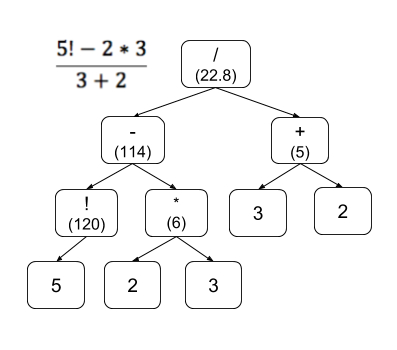
\includegraphics[width=0.45\textwidth]{image/ParseTrees1.png} &
		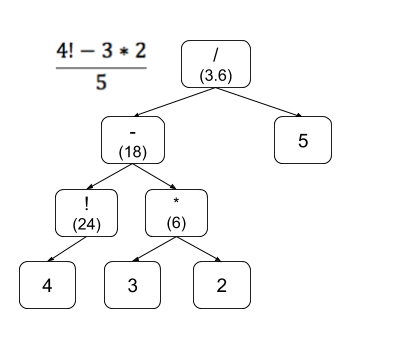
\includegraphics[width=0.45\textwidth]{image/ParseTrees2.png}
	\end{tabular}
   \caption{Two mathematical expressions and their parse
     trees. Consider the left tree, which corresponds to the
     expression $(5!-2*3)/(3+2)$. The root node corresponds to the
     operation that is evaluated last, which is division : $/$. The
     left subtree corresponds to the sub-expression $(5!-2*3)$ and the
     right subtree corresponds to the sub-epression $(3+2)$. The
     values written in parenthasis $(114)$,$(5)$ are the values of
     subexpressions. By taking the ratio $114/5$ we get the value of
     the root $(22.6)$}
   \label{fig:parse_tree}
\end{figure}

\section{Statistical Study of the Effectiveness of hints}

We used a controlled study methodology to quantify the effect of our
hints on student performance. For four of the weekly assignments, we
randomly placed each student with equal odds into a case group or a
control group. We refer to those students as case students and control
students.  We use the term {\em session} to refer to the record of a
single student working on a single problem. We use the term {\em
  attempt} to refer to a single attempted answer a student sends to
the edX system.

We filter out case student sessions in which the student did not
receive a hint, either because her attempt did not trigger a hint or
because she did not click on the ``show hint'' button.  To make the
control set as similar as possible, we filter out control student
sessions whose attempts would not have triggered a hint had they been
in the case set.

To quantify the effect we use three measures:
\begin{itemize}
\item {\bf Number of attempts:} Students were given an unlimited number of attempts. In most cases, students made attempts until they found a correct answer. We use the number of attempts to quantify the degree of difficulty experienced by the student when solving the problem.

\item {\bf Total attempt time:} In addition to the number of attempts, we estimate the total amount of time the student spent on the problem. Students periodically take a break and continue after a few hours or days, we reduce the effect of such time gaps on our estimate by eliminating any time gap longer than ten minutes.
\item {\bf Problem grade in final:} Most homework assignments have a corresponding problem in the final exam. We use the grade of said problem to quantify the long-term effect of receiving hints. 
\end{itemize}

Our goal is to establish that the hints we produce have a positive effect on learning. The null hypothesis that we aim to reject is that hints have no effect. We consider the potential effect at three different time scales. The {\em within problem effect} is the effect of receiving a hint when attempting to answer a problem on the performance of students {\em on the same problem}. The {\em within assignment effect} is the effect of receiving a hint when attempting to solve a problem on the performance of students on later problem {\em within the same assignment}. Finally, the {\em long-term effect} is the effect of receiving hints during an assignment on the performance of the student on questions on the same material in the final exam.

We found no statistically significant effect for either the within problem or the long-term effect. On the other hand, we found a significant effect on the same assignment. We present the analysis and then discuss.

\subsection{Within problem effect}

Our first attempt was to evaluate whether receiving a hint while
working on a problem helps the student solve the problem faster than otherwise.

We consider each problem within the four weeks of our evaluation. For
each problem, we compute the number of attempts and the length of time
each student spent on the problem. We compare the number of attempts
and the length of time for each problem between the case students who
received at least one hint and the control students that would have
received a hint were they in the case group.

Analysis of the results using a t-test failed to detect a
statistically significant difference between the case and the
control. 

\iffalse
\begin{figure}[ht]
  \centering
   \begin{tabular}{c c}
  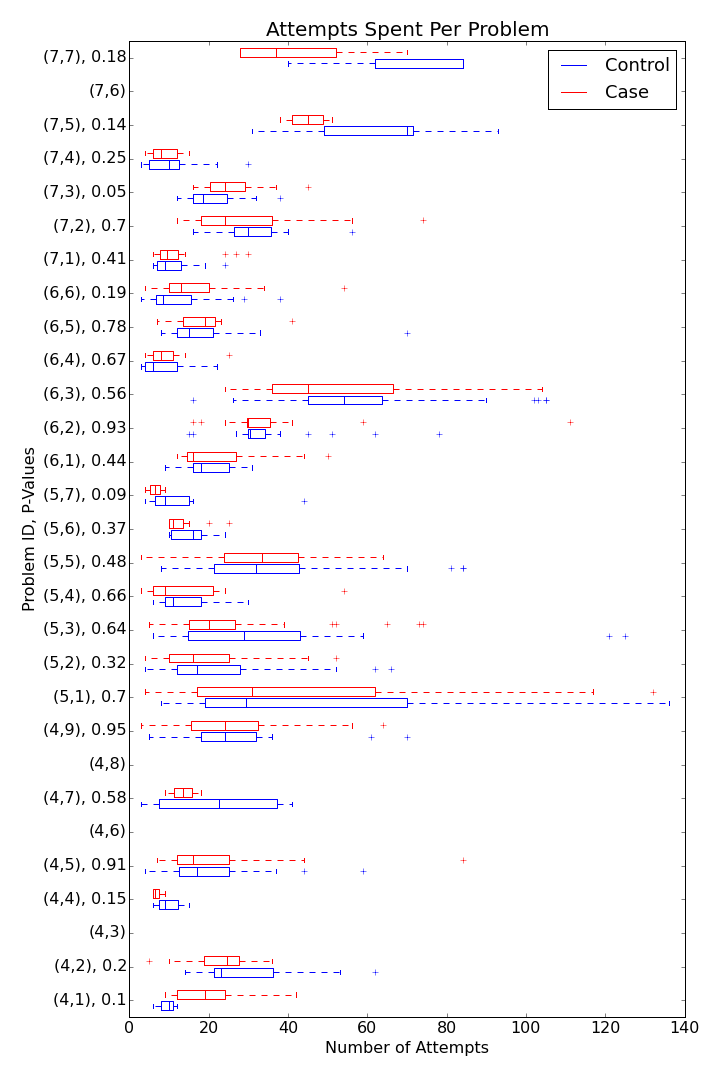
\includegraphics[width=0.48\textwidth]{image/problem_tries.png} & 
  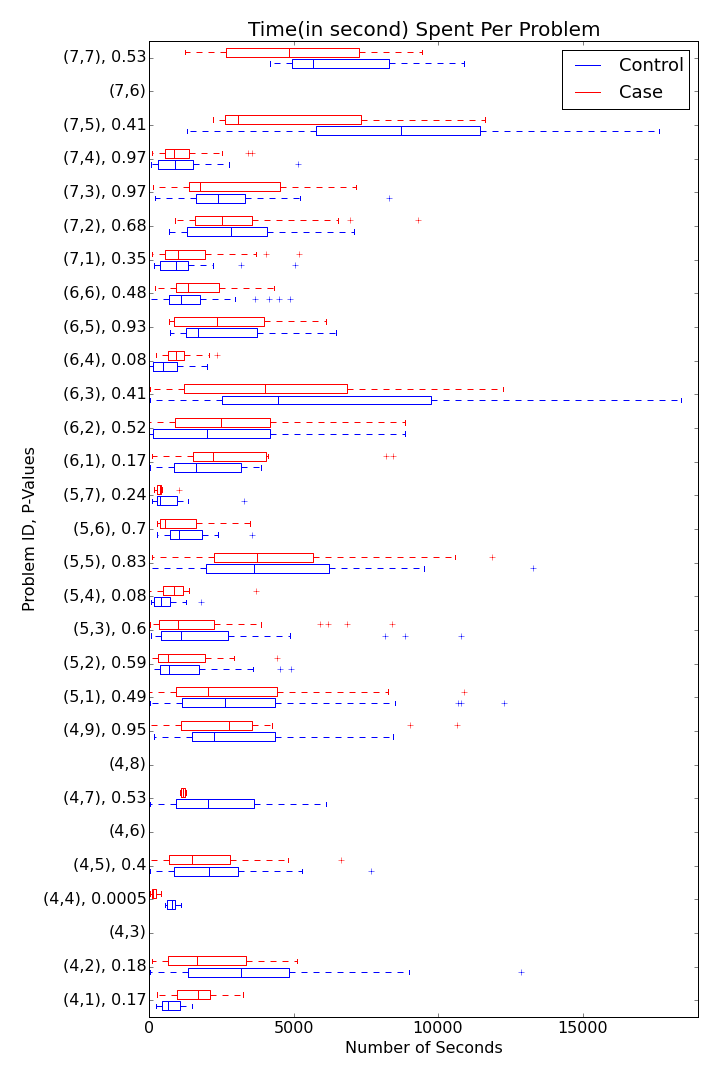
\includegraphics[width=0.48\textwidth]{image/problem_time.png}
  \end{tabular}
  \caption{Two box plots of the number of attempts and number of seconds spent on each problem with hints. The problems with no hint written have no data present. Problem (4,3), for example, has no hint sent, and therefore has no data on graph. Each problem has a control set and a case set. It is hard to tell which group of students spent more attempts or more time than the other. The axis label also shows the p-value of the two sided t-test. Most of the problems have very high p-value and therefore the result is not significant to draw conclusion.}
   \label{fig:tries_analysis}
\end{figure}
\fi

\subsection{Within assignment effect}

Our second attempt was to evaluate whether case students that received a hint while
working on an assignment helps the student solve later problems within
the same assignment more quickly that students 
faster than otherwise.

We define ``problem with hint'' as follows. For the case student, a
problem with hint is a problem where a hint was sent to the student who then chose to view it. For a control student, it is a problem for which a hint would have been sent, had the student been in the case.

We consider only sessions that have at least one problem with
hint. For each such session, we consider all of the problems {\em
  without hint} that the student worked on after working on the
problem with hint. We call these problems the ``downstream'' problems.

For example, suppose the student solved an assignment of 9 problems in the following order $\{ 1, 4, 3, 2, 6, 5, 7, 8, 9\}$. This student received at least one hint on problems $\{3, 5, 7\}$. Therefore, the downstream problems for this session are $\{2, 6, 8, 9\}$.

For each session, we compute the number of attempts (and the amount of time) spent on each of the downstream problems. We partition these measurements into two populations depending on whether the student was in the case or the control. See Figure \ref{fig:prob_tries_analysis}. We perform a two sided t-test on each of the problem. We observed that 20 out of 25 problems have p-value less than $5\%$ and 4 problems have no hints sent.

\begin{figure}[ht]
  \centering
  \begin{tabular}{c c}
  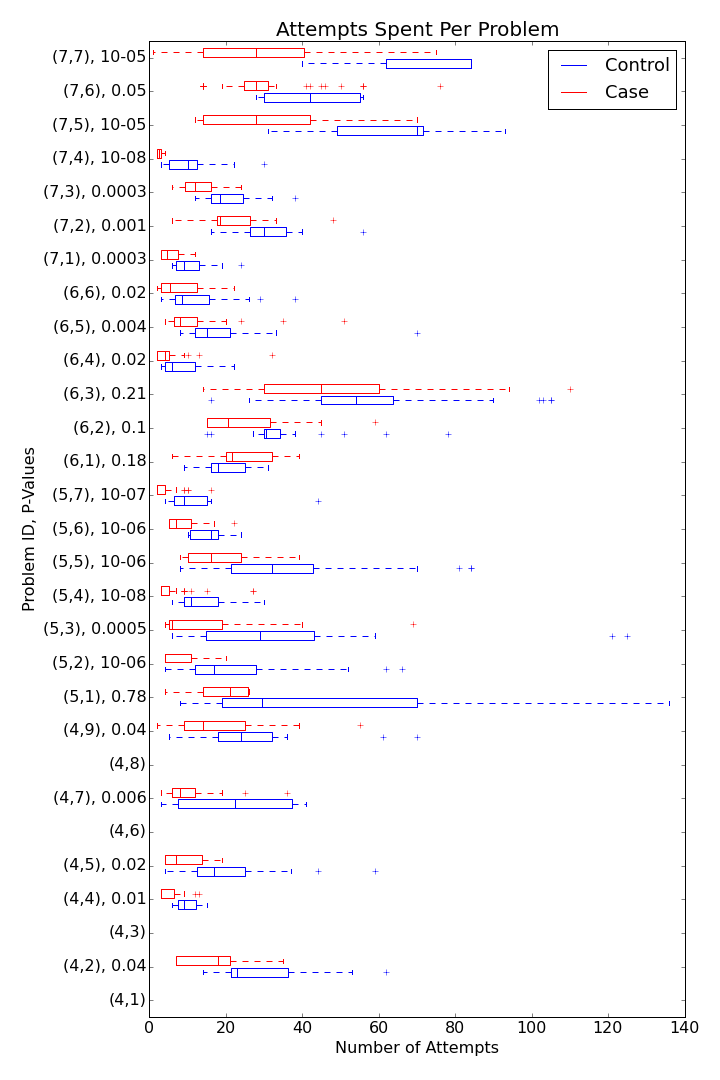
\includegraphics[width=0.5\textwidth]{image/problem_tries_downstream.png} & 
  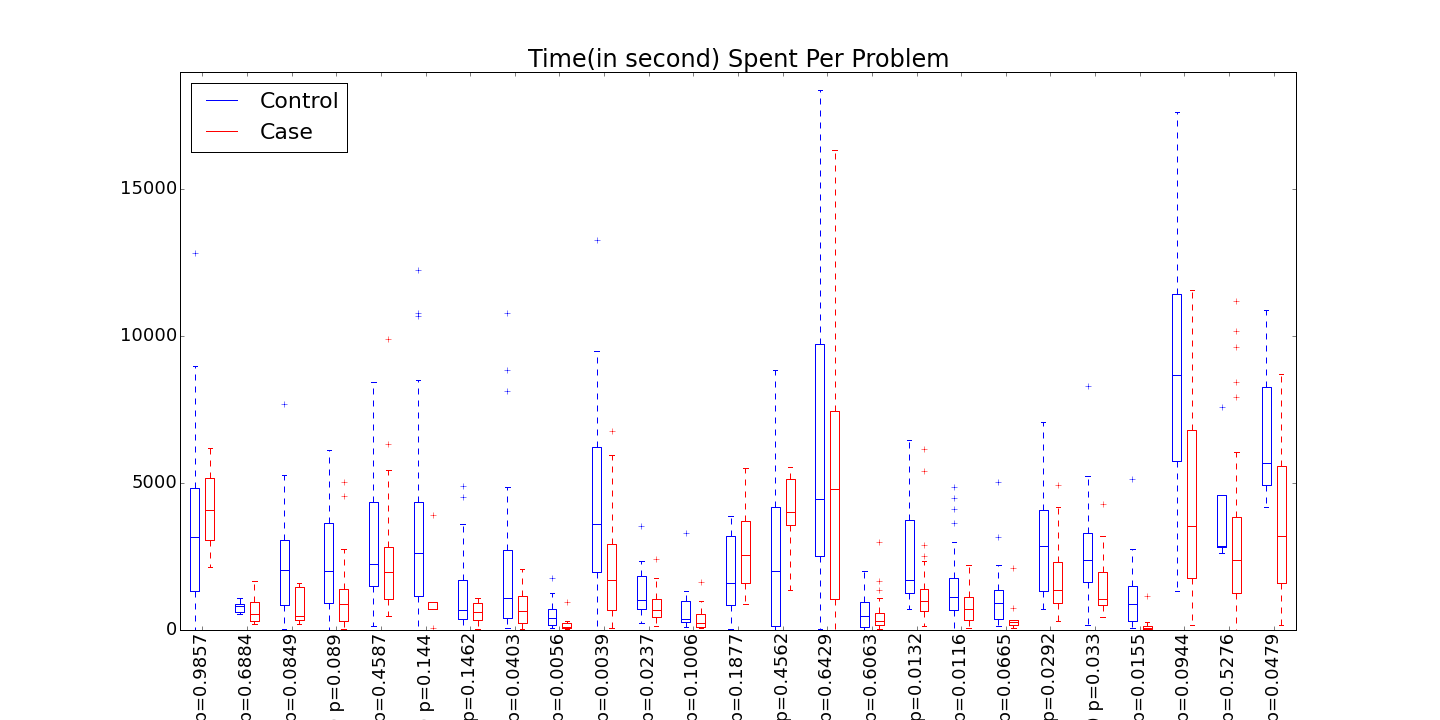
\includegraphics[width=0.5\textwidth]{image/problem_time_downstream.png}
  \end{tabular}
  \caption{Box plots of the number of attempts and length of time spent on downstream problems for control students and case students. The problems with no hint sent is left blank on the graph. It is clearly shown that the control group spent more attempts and more time than case students on almost all problems with hint sent. The axis label also shows the p-value being very small. Only a few problems have p-value more than $5\%$. For some of the problems we don't have hints sent, there is no box plots presented.}
   \label{fig:prob_tries_analysis}
\end{figure}

We also did similar analysis of student effort on each assignment as a
whole. We consider problems that have been attempted after a the first
problem on which the student recieved a hint. We call these problems
``downstream'' problems. We define the average number of attempts(or
length of time) spent by control group on each problem in the
assignment as the {\em baseline}. Then, for each student in the case
group, we measure the sum of attempts (or length of time) for the
downstream problems. We compute the difference between this sum and
the sum of the corresponding baselines. The result is the difference
in the number of attempts between the case student and the average
control. If the difference is negative, it means the case student
solved the downstream problems within a smaller number of attempts.
We show the histograms of the differences in Figure
\ref{fig:downstream_tries_analysis} and Figure
\ref{fig:downstream_time_analysis}. The plots show that in most cases
the result of getting a hint is a reduction in number of attempts, or
amount of time spent, on the downstream problems comparing to control
students.

\begin{figure}[ht]
\centering

\includegraphics[width=0.9\textwidth]{image/assignment_tries_downstream.png}
\caption{The distribution of the attempt differences between case student and the control students. Each subplot corresponds to the distribution of an assignment. All four graphs have distribution with negative means, which means that the control students spent more attempts comparing to the case students.}
    \label{fig:downstream_tries_analysis}
\end{figure}

\begin{figure}[ht]
\centering
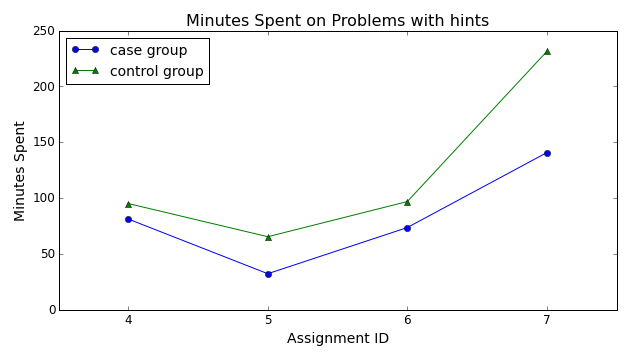
\includegraphics[width=0.9\textwidth]{image/assignment_time_downstream.png}
\caption{The distribution of time (in seconds) differences between case students and control students. All distribution have negative means, showing that control students spend more time on each assignment than the case students. The results are consistent with Figure \ref{fig:downstream_tries_analysis}}
    \label{fig:downstream_time_analysis}
\end{figure}

We perform a one sample t-test with null hypothesis that the mean of
the attempt differences (or the time differences) should be
zero. Table \ref{tab:no_hint} and Table \ref{tab:no_hint_time} show
that we have small p-value for each of the assignment. Therefore, we
reject the null hypothesis and conclude that case students and control
students have significantly different performance and that case
students spend less attempts and less time on homework problems
comparing to control students. This analysis shows that the adaptive
hint system helps students perform better in homework problems that
come after the hints.


\begin{table}[th]
\caption{The table listed the attempt differences between control students and case students. For each of the four weeks, the control students spent more attempts than the case students. The p-value of the one sample t-test is also presented in the table. The p-values are all extremly small that we can reject the null hypothesis and conclude that the performance of case students and control students are significantly different.}
\begin{center}
  \begin{tabular}{| c | c | c | c | c | c |}
  \hline
    Week & Number& Mean of total & Std of total &  P-Value of a &Average amount \\
    Number & of & attempts & attempts & two sided one & of total attempt spent\\
     & instances & differences & differences & sample t-test & on assignment   \\ \hline
	4 & 43 & -22.234 & 26.825 & $3.16 * 10^{-6}$ & 11.604\\
	5 & 81 & -43.128 & 35.508 & $2.058 * 10 ^{-17}$ & 18.03\\
	6 & 64 & -19.955 & 29.943 & $1.641 * 10^{-6}$ &  18.52\\
	7 & 55 & -86.785 & 39.392 & $2.250 * 10^{-22}$ & 20.838\\
	\hline
  \end{tabular}
  \label{tab:no_hint}
  \end{center}
\end{table}

\begin{table}
\caption{The table listed the time differences (in minutes) between the control students and the case students. Similar to Table \ref{tab:no_hint}, case students spent less time on all assignments comparing to control students. The p-values of the one sample t-test are also very small. Only assignment 4 has p-value a little over $5\%$.}
\begin{center}
  \begin{tabular}{| c | c | c | c | c | c |}
    \hline
    Week & Number& Mean of total & Std of total &  P-Value of a &Average amount \\
    Number & of & time(seconds) & time(seconds) & two sided one & of total time spent\\
     & instances & differences & differences & sample t-test & on assignment   \\ \hline
	4 & 41 & -833.087 & 2983.083 & 0.085 & 1035.228\\
	5 & 62 & -1989.48 &1887.724 & $1.761 * 10^{-11}$ & 1035.228\\
	6 & 58 & -1396.852 & 3850.474 & 0.0082 & 1610.531 \\
	7 & 53 & -5438.16 & 5671.409 & $6.77 * 10^{-9}$ & 1886.64\\
	\hline
  \end{tabular}
  \label{tab:no_hint_time}
  \end{center}
\end{table}



\subsection{Long term effect}
Final scores play an important role as to evaluate the learning outcome of students. We examine whether hints have effect on students' final score.

The problems in the final exam aim to examine students understanding
of different topics learned in lectures. Each of these topics have a
collection of homework problems for students to practice.

\iffalse
We map a set of homework problems for each of the final problem as shown in Table \ref{tab:map}.

\begin{table}[h]
\caption{Each final problem on the left has a set of corresponding homework problems on the right. The problem ID is in the format of week number and problem number. For example, (4,1) means problem 1 of assignment in week 4.}
\begin{center}
  \begin{tabular}{ c | c }
   Final Problem & Homework Problem IDs \\ \hline
	3 & (4,1), (4,2) \\
	4 & (5,1), (5,2), (5,3), (5,4) \\
    5 & (6,4) \\
    6 & (6,6) \\
    7 & (6,2), (6,3) \\
    8 & (8,3), (8,4), (8,5), (8,6) \\ \hline
  \end{tabular}
  \label{tab:map}
  \end{center}
\end{table}
\fi
For each final problem, we consider the corresponding assignment. We
split students based on the control and case group of the
corresponding assignment. We compare control and case students on
their final score for each final problem. The data does not support
any conclusion from this analysis.

\iffalse
See Figure \ref{fig:final_compare_all}. It is hard to tell which group of students perform better than the other. The p-values are not small enough and we conclude that the effect of hints on final scores is non-detectable.


\begin{figure}[h]
\centering
\caption{Box plot of final score of both control group and case group for each final problem. The data points are labeled with p-value of a two-tailed t-test. We don't see a very clear advantage on either of the control or case. The p-values are also not small enough for us to reject the null hypothesis.}
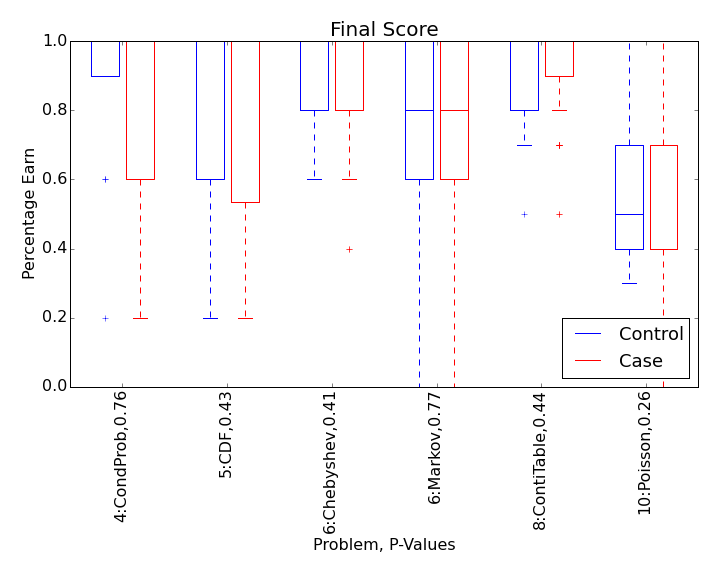
\includegraphics[width=0.9\linewidth]{image/final_boxPlot.png}
\label{fig:final_compare_all}
\end{figure}
\fi


\section{Conclusions and future work}

We designed and deployed an adaptive hint system for web-based
homework. Our controlled study shows that adaptive hints have a
significant positive effect on student performance.

The effect for which we have strong evidence is the effect of
recieving a hint while solving a problem on the performance of the
student on the cumulative effort of the student on the following
problems in the same assignment. We interpret this effect to mean that
the hint gave the student a better understanding of the problem
domain, and that this better understanding manifested itself when they
were working on other problems in the same domain, even though they
did not recieve hints on those problems.

We found some evidence that the recieving a hint effects student
performance on a single problem. This evidence is much weaker than the
evidence for the cumulative effort. This is not surprising because we
expect a strong correlation between the effects on different problems,
and this correlation is not captured when analyzing individual
problems.

We performed other tests for which we found no significant effect:
\begin{enumerate}
\item There was no significant effect of recieving a hint on the
  performanc of the student on the **same** problem.
\item We could find no significant effect of recieving effects on
  performance on the final exam.
\end{enumerate}

We are encouraged by the results of this study and plan to reuse and
refine the system in future offerings of the course, both in our
university and as an Online offerng on edX.

\bibliographystyle{splncs}
\bibliography{bibtxt}



\end{document}
